\section{Алгоритм на основе восходящего анализа}

Традиционно, алгоритмы, применяемые для анализа языков программирования как раз умеют строить дерево разбора --- то, что нам надо.
Только нам бы лес.
Вот и посмотрим, как это можно сделать.

Сперва поговорим про классический синтаксический анализ, потом про его адаптацию к анализу графов.

\subsection{Восходящий синтаксический анализ}

LR(k) --- алгоритм восходящего синтаксического анализа. 
Идея заключается в следующем: входная последовательность символов считывается слева направо с попутным добавлением в стек и выполнением сворачивания --- замены последовательности терминалов и нетерминалов, лежащих наверху стека, на нетерминал, если существует соответствующее правило в исходной грамматике.

\begin{definition}
Слот (item) --- правило грамматики, в правой части которого имеется точка, отделяющая уже разобранную часть правила (слева от точки) от того, что еще предстоит распознать (справа от точки).
\end{definition}

\begin{definition}
LR-автомат --- автомат с магазинной памятью, состояния которого задаются ``слотами'', также он имеет следующий набор инструкций: \\
1. shift p --- прочитать следующий символ входной последовательности, положив его в стек, и перейти в состояние p \\
2. reduce k --- применить k-ое правило грамматики, правая часть которого уже лежит на стеке: снимаем правую часть и кладём левую часть
\end{definition}

\begin{definition}
Предпросмотр --- метод, применяемый в синтаксическом анализе. Заключается в следующем: устанавливается максимальное количество входящих символов, которое может быть использовано анализатором для решения того, какое правило использовать (в случае восходящего анализа: к какому правилу нужно свернуться).
\end{definition}

\begin{definition}
Управляющая таблица --- таблица, которая для всех состояний LR-автомата содержит: инструкции для выполнения, если на вершине стека --- терминал (при этом в случае LR(k) в каждой ячейке может находиться не более одной инструкции), номер состояния, в которое нужно перейти, если на вершине стека --- нетерминал.
\end{definition}

Когда в текущем состоянии '.' стоит в конце, мы можем выполнить reduce-инструкцию и перейти в новое состояние. Однако при этом могут возникать следующие конфликты:
\begin{itemize}
\item shift-reduce --- ситуация, когда не понятно, читать ли следующий символ или выполнить reduce. Например, если правая часть одного из правил является префиксом правой части другого правила: $N \rightarrow w, M \rightarrow ww'$.
\item reduce-reduce --- ситуация, когда не понятно, к какому правилу нужно применить reduce. Например, если есть два правила с одинаковыми правыми частями: $N \rightarrow w, M \rightarrow w$.
\end{itemize}

Возьмем следующую грамматику:
\begin{align*}
0) S & \rightarrow a S b S \\
1) S & \rightarrow \varepsilon
\end{align*}

Расширим вышеупомянутую грамматику, добавив новый стартовый нетерминал S', и далее будем работать с этой расширенной грамматикой:
\begin{align*}
0) & S \rightarrow a S b S \\
1) & S \rightarrow \varepsilon \\
2) & S' \rightarrow S \$
\end{align*}

\begin{definition}
Замыкание --- обобщение понятия ``item'', заключающееся в добавлении для каждого item'а вида $N \rightarrow \alpha.M\beta$ item'ов вида $M \rightarrow .\gamma$
\end{definition}

\begin{definition}
Ядро --- исходный item, до применения к нему замыкания.
\end{definition}

\begin{example}
Пример ядра и замыкания. 

Возьмем правило 2 нашей грамматики, предположим, что мы только начинаем разбирать данное правило.

Ядром в таком случае является item исходного правила: $S' \rightarrow .S \$$

При замыкании добавятся ещё два item'a с правилами по выводу нетерминала 'S', поэтому получаем три item'a: $S' \rightarrow .S\$$, $S \rightarrow .aSbS$ и $S \rightarrow .\varepsilon$
\end{example}

\begin{example}
Пример построения LR-автомата для нашей грамматики с применением замыкания.
\begin{enumerate}
\item Добавляем стартовое состояние: item правила 0 и его замыкание (вместо item'a $S \rightarrow .\varepsilon$ будем писать $S \rightarrow .$). \\ \\
\tikzset{every picture/.style={line width=0.75pt}}
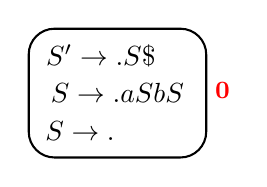
\begin{tikzpicture}[x=0.75pt,y=0.75pt,yscale=-1,xscale=1]
%Rounded Rect
\draw   (139.33,32.07) .. controls (139.33,25.22) and (144.89,19.67) .. (151.74,19.67) -- (212.44,19.67) .. controls (219.29,19.67) and (224.85,25.22) .. (224.85,32.07) -- (224.85,69.3) .. controls (224.85,76.15) and (219.29,81.71) .. (212.44,81.71) -- (151.74,81.71) .. controls (144.89,81.71) and (139.33,76.15) .. (139.33,69.3) -- cycle ;
\draw (174.09,32.69) node  [align=left] {$S' \rightarrow .S\$$};
\draw (182.09,50.69) node  [align=left] {$S \rightarrow .aSbS$};
\draw (164,69) node  [align=left] {$S \rightarrow .$};
\draw (232.67,49.33) node  [align=left] {\textbf{{\small \textcolor{red}{0}}}};
\end{tikzpicture}

\item По 'S' добавляем переход из стартового состояния в новое состояние 1. \\ \\
\tikzset{every picture/.style={line width=0.75pt}}
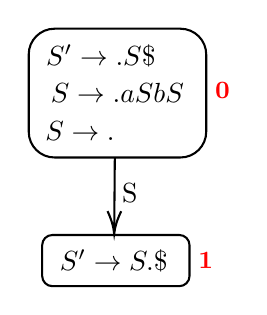
\begin{tikzpicture}[x=0.75pt,y=0.75pt,yscale=-1,xscale=1]
%Rounded Rect
\draw   (139.33,32.07) .. controls (139.33,25.22) and (144.89,19.67) .. (151.74,19.67) -- (212.44,19.67) .. controls (219.29,19.67) and (224.85,25.22) .. (224.85,32.07) -- (224.85,69.3) .. controls (224.85,76.15) and (219.29,81.71) .. (212.44,81.71) -- (151.74,81.71) .. controls (144.89,81.71) and (139.33,76.15) .. (139.33,69.3) -- cycle ;
%Rounded Rect
\draw   (145.81,123.98) .. controls (145.81,121.26) and (148.02,119.05) .. (150.74,119.05) -- (211.87,119.05) .. controls (214.6,119.05) and (216.81,121.26) .. (216.81,123.98) -- (216.81,138.78) .. controls (216.81,141.51) and (214.6,143.72) .. (211.87,143.72) -- (150.74,143.72) .. controls (148.02,143.72) and (145.81,141.51) .. (145.81,138.78) -- cycle ;
%Straight Lines 
\draw    (180.81,81.92) -- (180.53,116.51) ;
\draw [shift={(180.51,118.51)}, rotate = 270.47] [color={rgb, 255:red, 0; green, 0; blue, 0 }  ][line width=0.75]    (10.93,-3.29) .. controls (6.95,-1.4) and (3.31,-0.3) .. (0,0) .. controls (3.31,0.3) and (6.95,1.4) .. (10.93,3.29)   ;
\draw (174.09,32.69) node  [align=left] {$S' \rightarrow .S\$$};
\draw (182.09,50.69) node  [align=left] {$S \rightarrow .aSbS$};
\draw (164,69) node  [align=left] {$S \rightarrow .$};
\draw (180.33,131.67) node  [align=left] {$S' \rightarrow S.\$$};
\draw (188,99) node  [align=left] {S};
\draw (232.67,49.33) node  [align=left] {\textbf{{\small \textcolor{red}{0}}}};
\draw (224.67,131.33) node  [align=left] {\textbf{{\small \textcolor{red}{1}}}};
\end{tikzpicture}

\item По '\$' добавляем переход из состояния 1 в новое состояние 2. \\ \\
\tikzset{every picture/.style={line width=0.75pt}}
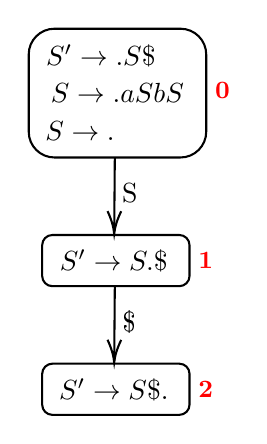
\begin{tikzpicture}[x=0.75pt,y=0.75pt,yscale=-1,xscale=1]
%Rounded Rect
\draw   (139.33,32.07) .. controls (139.33,25.22) and (144.89,19.67) .. (151.74,19.67) -- (212.44,19.67) .. controls (219.29,19.67) and (224.85,25.22) .. (224.85,32.07) -- (224.85,69.3) .. controls (224.85,76.15) and (219.29,81.71) .. (212.44,81.71) -- (151.74,81.71) .. controls (144.89,81.71) and (139.33,76.15) .. (139.33,69.3) -- cycle ;
%Rounded Rect
\draw   (145.81,123.98) .. controls (145.81,121.26) and (148.02,119.05) .. (150.74,119.05) -- (211.87,119.05) .. controls (214.6,119.05) and (216.81,121.26) .. (216.81,123.98) -- (216.81,138.78) .. controls (216.81,141.51) and (214.6,143.72) .. (211.87,143.72) -- (150.74,143.72) .. controls (148.02,143.72) and (145.81,141.51) .. (145.81,138.78) -- cycle ;
%Rounded Rect
\draw   (145.81,185.98) .. controls (145.81,183.26) and (148.02,181.05) .. (150.74,181.05) -- (211.87,181.05) .. controls (214.6,181.05) and (216.81,183.26) .. (216.81,185.98) -- (216.81,200.78) .. controls (216.81,203.51) and (214.6,205.72) .. (211.87,205.72) -- (150.74,205.72) .. controls (148.02,205.72) and (145.81,203.51) .. (145.81,200.78) -- cycle ;
%Straight Lines 
\draw    (180.81,81.92) -- (180.53,116.51) ;
\draw [shift={(180.51,118.51)}, rotate = 270.47] [color={rgb, 255:red, 0; green, 0; blue, 0 }  ][line width=0.75]    (10.93,-3.29) .. controls (6.95,-1.4) and (3.31,-0.3) .. (0,0) .. controls (3.31,0.3) and (6.95,1.4) .. (10.93,3.29)   ;
%Straight Lines 
\draw    (180.81,143.92) -- (180.53,178.51) ;
\draw [shift={(180.51,180.51)}, rotate = 270.47] [color={rgb, 255:red, 0; green, 0; blue, 0 }  ][line width=0.75]    (10.93,-3.29) .. controls (6.95,-1.4) and (3.31,-0.3) .. (0,0) .. controls (3.31,0.3) and (6.95,1.4) .. (10.93,3.29)   ;
\draw (174.09,32.69) node  [align=left] {$S' \rightarrow .S\$$};
\draw (182.09,50.69) node  [align=left] {$S \rightarrow .aSbS$};
\draw (164,69) node  [align=left] {$S \rightarrow .$};
\draw (180.33,131.67) node  [align=left] {$S' \rightarrow S.\$$};
\draw (180.33,193.67) node  [align=left] {$S' \rightarrow S\$.$};
\draw (188,99) node  [align=left] {S};
\draw (188,161) node  [align=left] {\$};
\draw (232.67,49.33) node  [align=left] {\textbf{{\small \textcolor{red}{0}}}};
\draw (224.67,131.33) node  [align=left] {\textbf{{\small \textcolor{red}{1}}}};
\draw (224.67,193.33) node  [align=left] {\textbf{{\small \textcolor{red}{2}}}};
\end{tikzpicture}

\item По 'a' добавляем переход из стартового состояния в новое состояние 3 и делаем его замыкание. Также добавляем переход по 'a' из этого состояния в себя же. \\ \\
\tikzset{every picture/.style={line width=0.75pt}}
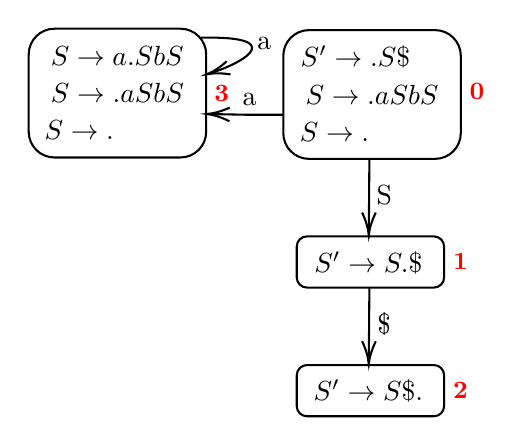
\begin{tikzpicture}[x=0.75pt,y=0.75pt,yscale=-1,xscale=1]
%Rounded Rect
\draw   (139.33,32.07) .. controls (139.33,25.22) and (144.89,19.67) .. (151.74,19.67) -- (212.44,19.67) .. controls (219.29,19.67) and (224.85,25.22) .. (224.85,32.07) -- (224.85,69.3) .. controls (224.85,76.15) and (219.29,81.71) .. (212.44,81.71) -- (151.74,81.71) .. controls (144.89,81.71) and (139.33,76.15) .. (139.33,69.3) -- cycle ;
%Rounded Rect
\draw   (145.81,123.98) .. controls (145.81,121.26) and (148.02,119.05) .. (150.74,119.05) -- (211.87,119.05) .. controls (214.6,119.05) and (216.81,121.26) .. (216.81,123.98) -- (216.81,138.78) .. controls (216.81,141.51) and (214.6,143.72) .. (211.87,143.72) -- (150.74,143.72) .. controls (148.02,143.72) and (145.81,141.51) .. (145.81,138.78) -- cycle ;
%Rounded Rect
\draw   (145.81,185.98) .. controls (145.81,183.26) and (148.02,181.05) .. (150.74,181.05) -- (211.87,181.05) .. controls (214.6,181.05) and (216.81,183.26) .. (216.81,185.98) -- (216.81,200.78) .. controls (216.81,203.51) and (214.6,205.72) .. (211.87,205.72) -- (150.74,205.72) .. controls (148.02,205.72) and (145.81,203.51) .. (145.81,200.78) -- cycle ;
%Rounded Rect 
\draw   (16.67,31.41) .. controls (16.67,24.56) and (22.22,19) .. (29.07,19) -- (89.77,19) .. controls (96.62,19) and (102.18,24.56) .. (102.18,31.41) -- (102.18,68.63) .. controls (102.18,75.48) and (96.62,81.04) .. (89.77,81.04) -- (29.07,81.04) .. controls (22.22,81.04) and (16.67,75.48) .. (16.67,68.63) -- cycle ;
%Straight Lines 
\draw    (180.81,81.92) -- (180.53,116.51) ;
\draw [shift={(180.51,118.51)}, rotate = 270.47] [color={rgb, 255:red, 0; green, 0; blue, 0 }  ][line width=0.75]    (10.93,-3.29) .. controls (6.95,-1.4) and (3.31,-0.3) .. (0,0) .. controls (3.31,0.3) and (6.95,1.4) .. (10.93,3.29)   ;
%Straight Lines 
\draw    (180.81,143.92) -- (180.53,178.51) ;
\draw [shift={(180.51,180.51)}, rotate = 270.47] [color={rgb, 255:red, 0; green, 0; blue, 0 }  ][line width=0.75]    (10.93,-3.29) .. controls (6.95,-1.4) and (3.31,-0.3) .. (0,0) .. controls (3.31,0.3) and (6.95,1.4) .. (10.93,3.29)   ;
%Straight Lines
\draw    (139.5,60.47) -- (122.5,60.47) -- (104.51,60.12) ;
\draw [shift={(102.51,60.09)}, rotate = 361.09000000000003] [color={rgb, 255:red, 0; green, 0; blue, 0 }  ][line width=0.75]    (10.93,-3.29) .. controls (6.95,-1.4) and (3.31,-0.3) .. (0,0) .. controls (3.31,0.3) and (6.95,1.4) .. (10.93,3.29)   ;
%Curve Lines
\draw    (99.51,23.34) .. controls (140.25,22.37) and (122.65,34.57) .. (104.22,40.43) ;
\draw [shift={(102.51,40.96)}, rotate = 343.53999999999996] [color={rgb, 255:red, 0; green, 0; blue, 0 }  ][line width=0.75]    (10.93,-3.29) .. controls (6.95,-1.4) and (3.31,-0.3) .. (0,0) .. controls (3.31,0.3) and (6.95,1.4) .. (10.93,3.29)   ;
\draw (174.09,32.69) node  [align=left] {$S' \rightarrow .S\$$};
\draw (182.09,50.69) node  [align=left] {$S \rightarrow .aSbS$};
\draw (164,69) node  [align=left] {$S \rightarrow .$};
\draw (180.33,131.67) node  [align=left] {$S' \rightarrow S.\$$};
\draw (180.33,193.67) node  [align=left] {$S' \rightarrow S\$.$};
\draw (59.33,32.33) node  [align=left] {$S \rightarrow a.SbS$};
\draw (59.42,50.02) node  [align=left] {$S \rightarrow .aSbS$};
\draw (41,68) node  [align=left] {$S \rightarrow .$};
\draw (188,99) node  [align=left] {S};
\draw (188,161) node  [align=left] {\$};
\draw (123,53) node  [align=left] {a};
\draw (130,26) node  [align=left] {a};
\draw (232.67,49.33) node  [align=left] {\textbf{{\small \textcolor{red}{0}}}};
\draw (224.67,131.33) node  [align=left] {\textbf{{\small \textcolor{red}{1}}}};
\draw (224.67,193.33) node  [align=left] {\textbf{{\small \textcolor{red}{2}}}};
\draw (109.67,50.33) node  [align=left] {\textbf{{\small \textcolor{red}{3}}}};
\end{tikzpicture}

\item По 'S' добавляем переход из состояния 3 в новое состояние 4. \\ \\
\tikzset{every picture/.style={line width=0.75pt}}
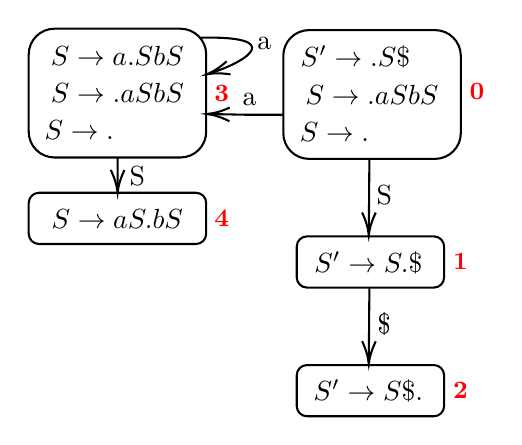
\begin{tikzpicture}[x=0.75pt,y=0.75pt,yscale=-1,xscale=1]
%Rounded Rect
\draw   (139.33,32.07) .. controls (139.33,25.22) and (144.89,19.67) .. (151.74,19.67) -- (212.44,19.67) .. controls (219.29,19.67) and (224.85,25.22) .. (224.85,32.07) -- (224.85,69.3) .. controls (224.85,76.15) and (219.29,81.71) .. (212.44,81.71) -- (151.74,81.71) .. controls (144.89,81.71) and (139.33,76.15) .. (139.33,69.3) -- cycle ;
%Rounded Rect
\draw   (145.81,123.98) .. controls (145.81,121.26) and (148.02,119.05) .. (150.74,119.05) -- (211.87,119.05) .. controls (214.6,119.05) and (216.81,121.26) .. (216.81,123.98) -- (216.81,138.78) .. controls (216.81,141.51) and (214.6,143.72) .. (211.87,143.72) -- (150.74,143.72) .. controls (148.02,143.72) and (145.81,141.51) .. (145.81,138.78) -- cycle ;
%Rounded Rect
\draw   (145.81,185.98) .. controls (145.81,183.26) and (148.02,181.05) .. (150.74,181.05) -- (211.87,181.05) .. controls (214.6,181.05) and (216.81,183.26) .. (216.81,185.98) -- (216.81,200.78) .. controls (216.81,203.51) and (214.6,205.72) .. (211.87,205.72) -- (150.74,205.72) .. controls (148.02,205.72) and (145.81,203.51) .. (145.81,200.78) -- cycle ;
%Rounded Rect 
\draw   (16.67,31.41) .. controls (16.67,24.56) and (22.22,19) .. (29.07,19) -- (89.77,19) .. controls (96.62,19) and (102.18,24.56) .. (102.18,31.41) -- (102.18,68.63) .. controls (102.18,75.48) and (96.62,81.04) .. (89.77,81.04) -- (29.07,81.04) .. controls (22.22,81.04) and (16.67,75.48) .. (16.67,68.63) -- cycle ;
%Rounded Rect
\draw   (16.67,102.98) .. controls (16.67,100.26) and (18.88,98.05) .. (21.6,98.05) -- (97.25,98.05) .. controls (99.97,98.05) and (102.18,100.26) .. (102.18,102.98) -- (102.18,117.78) .. controls (102.18,120.51) and (99.97,122.72) .. (97.25,122.72) -- (21.6,122.72) .. controls (18.88,122.72) and (16.67,120.51) .. (16.67,117.78) -- cycle ;
%Straight Lines 
\draw    (180.81,81.92) -- (180.53,116.51) ;
\draw [shift={(180.51,118.51)}, rotate = 270.47] [color={rgb, 255:red, 0; green, 0; blue, 0 }  ][line width=0.75]    (10.93,-3.29) .. controls (6.95,-1.4) and (3.31,-0.3) .. (0,0) .. controls (3.31,0.3) and (6.95,1.4) .. (10.93,3.29)   ;
%Straight Lines 
\draw    (180.81,143.92) -- (180.53,178.51) ;
\draw [shift={(180.51,180.51)}, rotate = 270.47] [color={rgb, 255:red, 0; green, 0; blue, 0 }  ][line width=0.75]    (10.93,-3.29) .. controls (6.95,-1.4) and (3.31,-0.3) .. (0,0) .. controls (3.31,0.3) and (6.95,1.4) .. (10.93,3.29)   ;
%Straight Lines
\draw    (139.5,60.47) -- (122.5,60.47) -- (104.51,60.12) ;
\draw [shift={(102.51,60.09)}, rotate = 361.09000000000003] [color={rgb, 255:red, 0; green, 0; blue, 0 }  ][line width=0.75]    (10.93,-3.29) .. controls (6.95,-1.4) and (3.31,-0.3) .. (0,0) .. controls (3.31,0.3) and (6.95,1.4) .. (10.93,3.29)   ;
%Curve Lines
\draw    (99.51,23.34) .. controls (140.25,22.37) and (122.65,34.57) .. (104.22,40.43) ;
\draw [shift={(102.51,40.96)}, rotate = 343.53999999999996] [color={rgb, 255:red, 0; green, 0; blue, 0 }  ][line width=0.75]    (10.93,-3.29) .. controls (6.95,-1.4) and (3.31,-0.3) .. (0,0) .. controls (3.31,0.3) and (6.95,1.4) .. (10.93,3.29)   ;
%Straight Lines
\draw    (59.51,81.05) -- (59.5,90) -- (59.5,96) ;
\draw [shift={(59.5,98)}, rotate = 270.03] [color={rgb, 255:red, 0; green, 0; blue, 0 }  ][line width=0.75]    (10.93,-3.29) .. controls (6.95,-1.4) and (3.31,-0.3) .. (0,0) .. controls (3.31,0.3) and (6.95,1.4) .. (10.93,3.29)   ;
\draw (174.09,32.69) node  [align=left] {$S' \rightarrow .S\$$};
\draw (182.09,50.69) node  [align=left] {$S \rightarrow .aSbS$};
\draw (164,69) node  [align=left] {$S \rightarrow .$};
\draw (180.33,131.67) node  [align=left] {$S' \rightarrow S.\$$};
\draw (180.33,193.67) node  [align=left] {$S' \rightarrow S\$.$};
\draw (59.33,32.33) node  [align=left] {$S \rightarrow a.SbS$};
\draw (59.42,50.02) node  [align=left] {$S \rightarrow .aSbS$};
\draw (41,68) node  [align=left] {$S \rightarrow .$};
\draw (59.33,110.67) node  [align=left] {$S \rightarrow aS.bS$};
\draw (188,99) node  [align=left] {S};
\draw (188,161) node  [align=left] {\$};
\draw (123,53) node  [align=left] {a};
\draw (130,26) node  [align=left] {a};
\draw (69,90) node  [align=left] {S};
\draw (232.67,49.33) node  [align=left] {\textbf{{\small \textcolor{red}{0}}}};
\draw (224.67,131.33) node  [align=left] {\textbf{{\small \textcolor{red}{1}}}};
\draw (224.67,193.33) node  [align=left] {\textbf{{\small \textcolor{red}{2}}}};
\draw (109.67,50.33) node  [align=left] {\textbf{{\small \textcolor{red}{3}}}};
\draw (109.67,110.33) node  [align=left] {\textbf{{\small \textcolor{red}{4}}}};
\end{tikzpicture}

\item По 'b' добавляем переход из состояния 4 в новое состояние 5 и делаем его замыкание. Также добавляем переход по 'a' из этого состояния в состояние 3. \\ \\
\tikzset{every picture/.style={line width=0.75pt}}
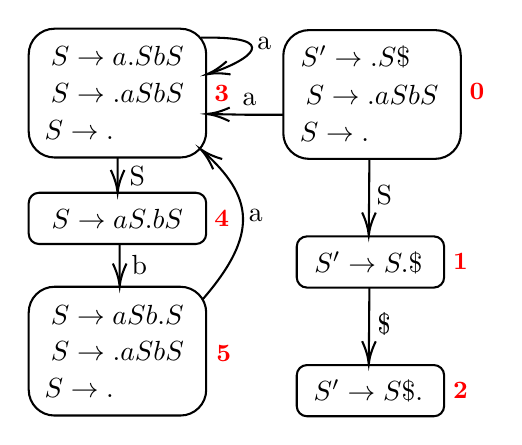
\begin{tikzpicture}[x=0.75pt,y=0.75pt,yscale=-1,xscale=1]
%Rounded Rect
\draw   (139.33,32.07) .. controls (139.33,25.22) and (144.89,19.67) .. (151.74,19.67) -- (212.44,19.67) .. controls (219.29,19.67) and (224.85,25.22) .. (224.85,32.07) -- (224.85,69.3) .. controls (224.85,76.15) and (219.29,81.71) .. (212.44,81.71) -- (151.74,81.71) .. controls (144.89,81.71) and (139.33,76.15) .. (139.33,69.3) -- cycle ;
%Rounded Rect
\draw   (145.81,123.98) .. controls (145.81,121.26) and (148.02,119.05) .. (150.74,119.05) -- (211.87,119.05) .. controls (214.6,119.05) and (216.81,121.26) .. (216.81,123.98) -- (216.81,138.78) .. controls (216.81,141.51) and (214.6,143.72) .. (211.87,143.72) -- (150.74,143.72) .. controls (148.02,143.72) and (145.81,141.51) .. (145.81,138.78) -- cycle ;
%Rounded Rect
\draw   (145.81,185.98) .. controls (145.81,183.26) and (148.02,181.05) .. (150.74,181.05) -- (211.87,181.05) .. controls (214.6,181.05) and (216.81,183.26) .. (216.81,185.98) -- (216.81,200.78) .. controls (216.81,203.51) and (214.6,205.72) .. (211.87,205.72) -- (150.74,205.72) .. controls (148.02,205.72) and (145.81,203.51) .. (145.81,200.78) -- cycle ;
%Rounded Rect 
\draw   (16.67,31.41) .. controls (16.67,24.56) and (22.22,19) .. (29.07,19) -- (89.77,19) .. controls (96.62,19) and (102.18,24.56) .. (102.18,31.41) -- (102.18,68.63) .. controls (102.18,75.48) and (96.62,81.04) .. (89.77,81.04) -- (29.07,81.04) .. controls (22.22,81.04) and (16.67,75.48) .. (16.67,68.63) -- cycle ;
%Rounded Rect
\draw   (16.67,102.98) .. controls (16.67,100.26) and (18.88,98.05) .. (21.6,98.05) -- (97.25,98.05) .. controls (99.97,98.05) and (102.18,100.26) .. (102.18,102.98) -- (102.18,117.78) .. controls (102.18,120.51) and (99.97,122.72) .. (97.25,122.72) -- (21.6,122.72) .. controls (18.88,122.72) and (16.67,120.51) .. (16.67,117.78) -- cycle ;
%Rounded Rect
\draw   (16.67,155.74) .. controls (16.67,148.89) and (22.22,143.33) .. (29.07,143.33) -- (89.77,143.33) .. controls (96.62,143.33) and (102.18,148.89) .. (102.18,155.74) -- (102.18,192.97) .. controls (102.18,199.82) and (96.62,205.37) .. (89.77,205.37) -- (29.07,205.37) .. controls (22.22,205.37) and (16.67,199.82) .. (16.67,192.97) -- cycle ;
%Straight Lines 
\draw    (180.81,81.92) -- (180.53,116.51) ;
\draw [shift={(180.51,118.51)}, rotate = 270.47] [color={rgb, 255:red, 0; green, 0; blue, 0 }  ][line width=0.75]    (10.93,-3.29) .. controls (6.95,-1.4) and (3.31,-0.3) .. (0,0) .. controls (3.31,0.3) and (6.95,1.4) .. (10.93,3.29)   ;
%Straight Lines 
\draw    (180.81,143.92) -- (180.53,178.51) ;
\draw [shift={(180.51,180.51)}, rotate = 270.47] [color={rgb, 255:red, 0; green, 0; blue, 0 }  ][line width=0.75]    (10.93,-3.29) .. controls (6.95,-1.4) and (3.31,-0.3) .. (0,0) .. controls (3.31,0.3) and (6.95,1.4) .. (10.93,3.29)   ;
%Straight Lines
\draw    (139.5,60.47) -- (122.5,60.47) -- (104.51,60.12) ;
\draw [shift={(102.51,60.09)}, rotate = 361.09000000000003] [color={rgb, 255:red, 0; green, 0; blue, 0 }  ][line width=0.75]    (10.93,-3.29) .. controls (6.95,-1.4) and (3.31,-0.3) .. (0,0) .. controls (3.31,0.3) and (6.95,1.4) .. (10.93,3.29)   ;
%Curve Lines
\draw    (99.51,23.34) .. controls (140.25,22.37) and (122.65,34.57) .. (104.22,40.43) ;
\draw [shift={(102.51,40.96)}, rotate = 343.53999999999996] [color={rgb, 255:red, 0; green, 0; blue, 0 }  ][line width=0.75]    (10.93,-3.29) .. controls (6.95,-1.4) and (3.31,-0.3) .. (0,0) .. controls (3.31,0.3) and (6.95,1.4) .. (10.93,3.29)   ;
%Straight Lines
\draw    (59.51,81.05) -- (59.5,90) -- (59.5,96) ;
\draw [shift={(59.5,98)}, rotate = 270.03] [color={rgb, 255:red, 0; green, 0; blue, 0 }  ][line width=0.75]    (10.93,-3.29) .. controls (6.95,-1.4) and (3.31,-0.3) .. (0,0) .. controls (3.31,0.3) and (6.95,1.4) .. (10.93,3.29)   ;
%Straight Lines  
\draw    (60.51,123.05) -- (60.5,132) -- (60.5,141.08) ;
\draw [shift={(60.5,143.08)}, rotate = 270] [color={rgb, 255:red, 0; green, 0; blue, 0 }  ][line width=0.75]    (10.93,-3.29) .. controls (6.95,-1.4) and (3.31,-0.3) .. (0,0) .. controls (3.31,0.3) and (6.95,1.4) .. (10.93,3.29)   ;
%Curve Lines
\draw    (100.5,149.38) .. controls (127.95,117.68) and (124.65,99.76) .. (100.98,78.35) ;
\draw [shift={(99.51,77.03)}, rotate = 401.35] [color={rgb, 255:red, 0; green, 0; blue, 0 }  ][line width=0.75]    (10.93,-3.29) .. controls (6.95,-1.4) and (3.31,-0.3) .. (0,0) .. controls (3.31,0.3) and (6.95,1.4) .. (10.93,3.29)   ;
\draw (174.09,32.69) node  [align=left] {$S' \rightarrow .S\$$};
\draw (182.09,50.69) node  [align=left] {$S \rightarrow .aSbS$};
\draw (164,69) node  [align=left] {$S \rightarrow .$};
\draw (180.33,131.67) node  [align=left] {$S' \rightarrow S.\$$};
\draw (180.33,193.67) node  [align=left] {$S' \rightarrow S\$.$};
\draw (59.33,32.33) node  [align=left] {$S \rightarrow a.SbS$};
\draw (59.42,50.02) node  [align=left] {$S \rightarrow .aSbS$};
\draw (41,68) node  [align=left] {$S \rightarrow .$};
\draw (59.33,110.67) node  [align=left] {$S \rightarrow aS.bS$};
\draw (59.33,156.67) node  [align=left] {$S \rightarrow aSb.S$};
\draw (59.42,174.35) node  [align=left] {$S \rightarrow .aSbS$};
\draw (41,192) node  [align=left] {$S \rightarrow .$};
\draw (188,99) node  [align=left] {S};
\draw (188,161) node  [align=left] {\$};
\draw (123,53) node  [align=left] {a};
\draw (130,26) node  [align=left] {a};
\draw (69,90) node  [align=left] {S};
\draw (70,133) node  [align=left] {b};
\draw (126,109) node  [align=left] {a};
\draw (232.67,49.33) node  [align=left] {\textbf{{\small \textcolor{red}{0}}}};
\draw (224.67,131.33) node  [align=left] {\textbf{{\small \textcolor{red}{1}}}};
\draw (224.67,193.33) node  [align=left] {\textbf{{\small \textcolor{red}{2}}}};
\draw (109.67,50.33) node  [align=left] {\textbf{{\small \textcolor{red}{3}}}};
\draw (109.67,110.33) node  [align=left] {\textbf{{\small \textcolor{red}{4}}}};
\draw (110.67,175.33) node  [align=left] {\textbf{{\small \textcolor{red}{5}}}};
\end{tikzpicture}

\item По 'S' добавляем переход из состояния 5 в новое состояние 6. Завершаем построение LR-автомата. \\ \\
\tikzset{every picture/.style={line width=0.75pt}}
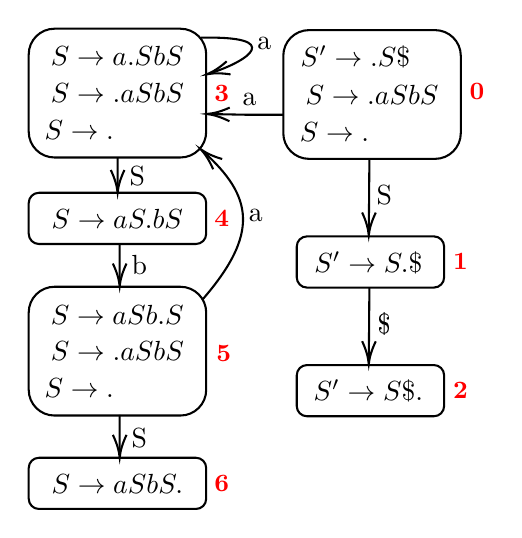
\begin{tikzpicture}[x=0.75pt,y=0.75pt,yscale=-1,xscale=1]
%Rounded Rect
\draw   (139.33,32.07) .. controls (139.33,25.22) and (144.89,19.67) .. (151.74,19.67) -- (212.44,19.67) .. controls (219.29,19.67) and (224.85,25.22) .. (224.85,32.07) -- (224.85,69.3) .. controls (224.85,76.15) and (219.29,81.71) .. (212.44,81.71) -- (151.74,81.71) .. controls (144.89,81.71) and (139.33,76.15) .. (139.33,69.3) -- cycle ;
%Rounded Rect 
\draw   (16.67,31.41) .. controls (16.67,24.56) and (22.22,19) .. (29.07,19) -- (89.77,19) .. controls (96.62,19) and (102.18,24.56) .. (102.18,31.41) -- (102.18,68.63) .. controls (102.18,75.48) and (96.62,81.04) .. (89.77,81.04) -- (29.07,81.04) .. controls (22.22,81.04) and (16.67,75.48) .. (16.67,68.63) -- cycle ;
%Rounded Rect
\draw   (16.67,155.74) .. controls (16.67,148.89) and (22.22,143.33) .. (29.07,143.33) -- (89.77,143.33) .. controls (96.62,143.33) and (102.18,148.89) .. (102.18,155.74) -- (102.18,192.97) .. controls (102.18,199.82) and (96.62,205.37) .. (89.77,205.37) -- (29.07,205.37) .. controls (22.22,205.37) and (16.67,199.82) .. (16.67,192.97) -- cycle ;
%Rounded Rect
\draw   (16.67,102.98) .. controls (16.67,100.26) and (18.88,98.05) .. (21.6,98.05) -- (97.25,98.05) .. controls (99.97,98.05) and (102.18,100.26) .. (102.18,102.98) -- (102.18,117.78) .. controls (102.18,120.51) and (99.97,122.72) .. (97.25,122.72) -- (21.6,122.72) .. controls (18.88,122.72) and (16.67,120.51) .. (16.67,117.78) -- cycle ;
%Rounded Rect
\draw   (16.67,230.65) .. controls (16.67,227.93) and (18.88,225.72) .. (21.6,225.72) -- (97.25,225.72) .. controls (99.97,225.72) and (102.18,227.93) .. (102.18,230.65) -- (102.18,245.45) .. controls (102.18,248.18) and (99.97,250.38) .. (97.25,250.38) -- (21.6,250.38) .. controls (18.88,250.38) and (16.67,248.18) .. (16.67,245.45) -- cycle ;
%Rounded Rect
\draw   (145.81,123.98) .. controls (145.81,121.26) and (148.02,119.05) .. (150.74,119.05) -- (211.87,119.05) .. controls (214.6,119.05) and (216.81,121.26) .. (216.81,123.98) -- (216.81,138.78) .. controls (216.81,141.51) and (214.6,143.72) .. (211.87,143.72) -- (150.74,143.72) .. controls (148.02,143.72) and (145.81,141.51) .. (145.81,138.78) -- cycle ;
%Rounded Rect
\draw   (145.81,185.98) .. controls (145.81,183.26) and (148.02,181.05) .. (150.74,181.05) -- (211.87,181.05) .. controls (214.6,181.05) and (216.81,183.26) .. (216.81,185.98) -- (216.81,200.78) .. controls (216.81,203.51) and (214.6,205.72) .. (211.87,205.72) -- (150.74,205.72) .. controls (148.02,205.72) and (145.81,203.51) .. (145.81,200.78) -- cycle ;
%Straight Lines 
\draw    (180.81,81.92) -- (180.53,116.51) ;
\draw [shift={(180.51,118.51)}, rotate = 270.47] [color={rgb, 255:red, 0; green, 0; blue, 0 }  ][line width=0.75]    (10.93,-3.29) .. controls (6.95,-1.4) and (3.31,-0.3) .. (0,0) .. controls (3.31,0.3) and (6.95,1.4) .. (10.93,3.29)   ;
%Straight Lines 
\draw    (180.81,143.92) -- (180.53,178.51) ;
\draw [shift={(180.51,180.51)}, rotate = 270.47] [color={rgb, 255:red, 0; green, 0; blue, 0 }  ][line width=0.75]    (10.93,-3.29) .. controls (6.95,-1.4) and (3.31,-0.3) .. (0,0) .. controls (3.31,0.3) and (6.95,1.4) .. (10.93,3.29)   ;
%Straight Lines
\draw    (59.51,81.05) -- (59.5,90) -- (59.5,96) ;
\draw [shift={(59.5,98)}, rotate = 270.03] [color={rgb, 255:red, 0; green, 0; blue, 0 }  ][line width=0.75]    (10.93,-3.29) .. controls (6.95,-1.4) and (3.31,-0.3) .. (0,0) .. controls (3.31,0.3) and (6.95,1.4) .. (10.93,3.29)   ;
%Straight Lines  
\draw    (60.51,123.05) -- (60.5,132) -- (60.5,141.08) ;
\draw [shift={(60.5,143.08)}, rotate = 270] [color={rgb, 255:red, 0; green, 0; blue, 0 }  ][line width=0.75]    (10.93,-3.29) .. controls (6.95,-1.4) and (3.31,-0.3) .. (0,0) .. controls (3.31,0.3) and (6.95,1.4) .. (10.93,3.29)   ;
%Straight Lines
\draw    (60.51,205.05) -- (60.5,214) -- (60.5,223.62) ;
\draw [shift={(60.5,225.62)}, rotate = 270.02] [color={rgb, 255:red, 0; green, 0; blue, 0 }  ][line width=0.75]    (10.93,-3.29) .. controls (6.95,-1.4) and (3.31,-0.3) .. (0,0) .. controls (3.31,0.3) and (6.95,1.4) .. (10.93,3.29)   ;
%Straight Lines
\draw    (139.5,60.47) -- (122.5,60.47) -- (104.51,60.12) ;
\draw [shift={(102.51,60.09)}, rotate = 361.09000000000003] [color={rgb, 255:red, 0; green, 0; blue, 0 }  ][line width=0.75]    (10.93,-3.29) .. controls (6.95,-1.4) and (3.31,-0.3) .. (0,0) .. controls (3.31,0.3) and (6.95,1.4) .. (10.93,3.29)   ;
%Curve Lines
\draw    (99.51,23.34) .. controls (140.25,22.37) and (122.65,34.57) .. (104.22,40.43) ;
\draw [shift={(102.51,40.96)}, rotate = 343.53999999999996] [color={rgb, 255:red, 0; green, 0; blue, 0 }  ][line width=0.75]    (10.93,-3.29) .. controls (6.95,-1.4) and (3.31,-0.3) .. (0,0) .. controls (3.31,0.3) and (6.95,1.4) .. (10.93,3.29)   ;
%Curve Lines
\draw    (100.5,149.38) .. controls (127.95,117.68) and (124.65,99.76) .. (100.98,78.35) ;
\draw [shift={(99.51,77.03)}, rotate = 401.35] [color={rgb, 255:red, 0; green, 0; blue, 0 }  ][line width=0.75]    (10.93,-3.29) .. controls (6.95,-1.4) and (3.31,-0.3) .. (0,0) .. controls (3.31,0.3) and (6.95,1.4) .. (10.93,3.29)   ;
\draw (174.09,32.69) node  [align=left] {$S' \rightarrow .S\$$};
\draw (59.33,32.33) node  [align=left] {$S \rightarrow a.SbS$};
\draw (59.33,156.67) node  [align=left] {$S \rightarrow aSb.S$};
\draw (59.33,110.67) node  [align=left] {$S \rightarrow aS.bS$};
\draw (59.33,238.33) node  [align=left] {$S \rightarrow aSbS.$};
\draw (180.33,131.67) node  [align=left] {$S' \rightarrow S.\$$};
\draw (180.33,193.67) node  [align=left] {$S' \rightarrow S\$.$};
\draw (59.42,50.02) node  [align=left] {$S \rightarrow .aSbS$};
\draw (41,68) node  [align=left] {$S \rightarrow .$};
\draw (182.09,50.69) node  [align=left] {$S \rightarrow .aSbS$};
\draw (164,69) node  [align=left] {$S \rightarrow .$};
\draw (59.42,174.35) node  [align=left] {$S \rightarrow .aSbS$};
\draw (41,192) node  [align=left] {$S \rightarrow .$};
\draw (126,109) node  [align=left] {a};
\draw (70,133) node  [align=left] {b};
\draw (123,53) node  [align=left] {a};
\draw (130,26) node  [align=left] {a};
\draw (69,90) node  [align=left] {S};
\draw (70,216) node  [align=left] {S};
\draw (188,99) node  [align=left] {S};
\draw (188,161) node  [align=left] {\$};
\draw (232.67,49.33) node  [align=left] {\textbf{{\small \textcolor{red}{0}}}};
\draw (109.67,50.33) node  [align=left] {\textbf{{\small \textcolor{red}{3}}}};
\draw (110.67,175.33) node  [align=left] {\textbf{{\small \textcolor{red}{5}}}};
\draw (224.67,131.33) node  [align=left] {\textbf{{\small \textcolor{red}{1}}}};
\draw (224.67,193.33) node  [align=left] {\textbf{{\small \textcolor{red}{2}}}};
\draw (109.67,110.33) node  [align=left] {\textbf{{\small \textcolor{red}{4}}}};
\draw (109.67,238.33) node  [align=left] {\textbf{{\small \textcolor{red}{6}}}};
\end{tikzpicture}
\end{enumerate}
\end{example}

\begin{example}
Пример управляющей таблицы для работы с построенным ранее LR-автоматом.

\begin{tabular}{|c|c|c|c||c|} 
    \hline & a & b & \$ & S \\ [0.5ex]
    \hline 0 & shift 3 & reduce 1 & reduce 1 & 1 \\
    \hline 1 & & & ACCEPT & \\
    \hline 2 & & & & \\
    \hline  3 & shift 3 & reduce 1 & reduce 1 & 4 \\
    \hline 4 & & shift 5 & & \\
    \hline 5 & shift 3 & reduce 1 & reduce 1 & 6 \\
    \hline 6 & & reduce 0 & reduce 0 & \\ [1ex] 
    \hline
\end{tabular}
\end{example}

\textbf{Ход работы LR-парсера.}
Пусть у нас есть входная строка, LR-автомат со стеком и управляющая таблица. \\
В начальный момент на стеке лежит стартовое состояние LR-автомата, позиция во входной строке соответствует её началу.
На каждом шаге анализируется текущий символ входа и текущее состояние, в котором находится автомат, и совершается одно из действий: 
\begin{itemize}
\item Если текущая позиция --- конец строки и в стеке --- стартовый нетерминал исходной грамматики, то успешно завершаем разбор.
\item Если в управляющей таблице нет инструкции для текущего состояния автомата и текущего символа на входе, то завершаем разбор с ошибкой.
\item Иначе выполняем инструкцию: \\
1) в случае shift --- кладем на стек текущий символ входа, сдвигая при этом текущую позицию, и номер нового состояния с переходом в него. \\
2) в случае reduce --- снимаем со стека 2k элементов: k состояний и k терминалов/нетерминалов (где k --- длина правой части правила, участвующего в свёртке), кладём на стек нетерминал левой части правила и, оказавшись в некотором состоянии, в котором мы были ранее (самое близкое к вершине из хранимых на стеке состояний), выполняем переход в новое состояние с добавлением его номера в стек, если в управляющей таблице пересечение текущего состояния и добавленного ранее нетерминала --- не пусто.
\end{itemize}

\begin{example}
Пример LR-разбора входного слова abab\$ из языка нашей грамматики с использованием построенных ранее LR-автомата и управляющей таблицы.
\begin{enumerate}
\item Начало разбора. На стеке --- стартовое состояние 0. \\ \\
Вход: \,
\begin{tabular}[c]{ |c|c|c|c|c| } 
    \hline \textcolor{red}{a} & b & a & b & \$ \\ \hline
\end{tabular}
\qquad Стек: \,
\begin{tabular}[c]{ |c|c } 
    \hline 0 & \\ \hline
\end{tabular}  
\\
\item Выполняем shift 3: сдвигаем указатель на входе, кладем на стек 'a', новое состояние 3 и переходим в него. \\ \\
Вход: \,
\begin{tabular}[c]{ |c|c|c|c|c| } 
    \hline a & \textcolor{red}{b} & a & b & \$ \\ \hline
\end{tabular}
\qquad Стек: \,
\begin{tabular}[c]{ |c|c|c|c } 
    \hline 0 & a & 3 & \\ \hline
\end{tabular}
\\ 
\item Выполняем reduce 1 (кладем на стек 'S'), кладем новое состояние 4 и переходим в него. \\ \\
Вход: \,
\begin{tabular}[c]{ |c|c|c|c|c| } 
    \hline a & \textcolor{red}{b} & a & b & \$ \\ \hline
\end{tabular}
\qquad Стек: \,
\begin{tabular}[c]{ |c|c|c|c|c|c } 
    \hline 0 & a & 3 & S & 4 & \\ \hline
\end{tabular}
\\ 
\item Выполняем shift 5: сдвигаем указатель на входе, кладем на стек 'b', новое состояние 5 и переходим в него. \\ \\
Вход: \,
\begin{tabular}[c]{ |c|c|c|c|c| } 
    \hline a & b & \textcolor{red}{a} & b & \$ \\ \hline
\end{tabular}
\qquad Стек: \,
\begin{tabular}[c]{ |c|c|c|c|c|c|c|c } 
    \hline 0 & a & 3 & S & 4 & b & 5 & \\ \hline
\end{tabular}
\\
\item Выполняем shift 3. \\ \\
Вход: \,
\begin{tabular}[c]{ |c|c|c|c|c| } 
    \hline a & b & a & \textcolor{red}{b} & \$ \\ \hline
\end{tabular}
\qquad Стек: \,
\begin{tabular}[c]{ |c|c|c|c|c|c|c|c|c|c } 
    \hline 0 & a & 3 & S & 4 & b & 5 & a & 3 & \\ \hline
\end{tabular}
\\
\item Выполняем reduce 1, кладем новое состояние 4 и переходим в него. \\ \\
Вход: \,
\begin{tabular}[c]{ |c|c|c|c|c| } 
    \hline a & b & a & \textcolor{red}{b} & \$ \\ \hline
\end{tabular}
\qquad Стек: \,
\begin{tabular}[c]{ |c|c|c|c|c|c|c|c|c|c|c|c } 
    \hline 0 & a & 3 & S & 4 & b & 5 & a & 3 & S & 4 & \\ \hline
\end{tabular}
\\
\item Выполняем shift 5. \\ \\
Вход: \,
\begin{tabular}[c]{ |c|c|c|c|c| } 
    \hline a & b & a & b & \textcolor{red}{\$} \\ \hline
\end{tabular}
\qquad Стек: \,
\begin{tabular}[c]{ |c|c|c|c|c|c|c|c|c|c|c|c|c|c } 
    \hline 0 & a & 3 & S & 4 & b & 5 & a & 3 & S & 4 & b & 5 & \\ \hline
\end{tabular}
\\
\item Выполняем reduce 1, кладем новое состояние 6 и переходим в него. \\ \\
Вход: \,
\begin{tabular}[c]{ |c|c|c|c|c| } 
    \hline a & b & a & b & \textcolor{red}{\$} \\ \hline
\end{tabular}
\qquad Стек: \,
\begin{tabular}[c]{ |c|c|c|c|c|c|c|c|c|c|c|c|c|c|c|c } 
    \hline 0 & a & 3 & S & 4 & b & 5 & a & 3 & S & 4 & b & 5 & S & 6 & \\ \hline
\end{tabular}
\\
\item Выполняем reduce 0 (снимаем со стека 8 элементов и кладем 'S'), оказываемся в состоянии 5 и делаем переход в новое состояние 6 с добавлением его на стек. \\ \\
Вход: \,
\begin{tabular}[c]{ |c|c|c|c|c| } 
    \hline a & b & a & b & \textcolor{red}{\$} \\ \hline
\end{tabular}
\qquad Стек: \,
\begin{tabular}[c]{ |c|c|c|c|c|c|c|c|c|c } 
    \hline 0 & a & 3 & S & 4 & b & 5 & S & 6 & \\ \hline
\end{tabular}
\\
\item Снова выполняем reduce 0, оказываемся в состоянии 0 и делаем переход в новое состояние 1 с добавлением его на стек. Заканчиваем разбор. \\ \\
Вход: \,
\begin{tabular}[c]{ |c|c|c|c|c| } 
    \hline a & b & a & b & \textcolor{red}{\$} \\ \hline
\end{tabular}
\qquad Стек: \,
\begin{tabular}[c]{ |c|c|c|c } 
    \hline 0 & S & 1 & \\ \hline
\end{tabular}
\end{enumerate}
\end{example}

На практике конфликты стараются решать ещё и на этапе генерации.
Да, реальные тулы могут сгенерировать парсер по неоднозначной грамматике: из переноса или свёртки выбирать перенос, из нескольких свёрток --- первую в каком-то порядке (обычно в порядке появления соответствующих продукций в грамматике).

Существует также модификация LR-разбора, которая называется SLR (Simple LR). 
Основная идея заключается в том, чтобы хранить в управляющей таблице reduce-инструкции только для тех терминалов, которые встречаются в правилах грамматики сразу после нетерминала, к которому выполняется свертка. 
Также существует LALR модификация (Look-Ahead LR).
В ней применяется склеивание нескольких состояний автомата, входные дуги которых имеют общие символы переходы, в одно состояние.
Данные модификации позволяют избежать большее число конфликтов, однако иногда могут иметь таблицы большего размера, чем в классическом LR.
Стоит отметить, что LALR(1)-парсер --- менее мощный, чем LR(1)-парсер, но более мощный, чем SLR(1)-парсер.

Немного про рекурсивно-восходящий анализ.

Но вообще, бывают обобщённые анализаторы, которые умеют обрабатывать все конфликты.

Томита --- вообще говоря не все граммтики, RNGLR~\cite{Scott:2006:RNG:1146809.1146810} --- все грамматики, но вообще говоря не за куб, а за произвольный полином, более продвинутый BRNGLR~\cite{!!!} --- все граммтики за куб.

Куча интересностей и подробностей~\cite{DBLP:phd/ethos/Economopoulos06}.

Общая идея --- объединение состояний. 

\begin{example}
Ну и пример с конфликтами и объединением состояний.
\end{example}


\subsection{Кс запросы}


Наша реализация~\cite{10.1007/978-3-319-41579-6_22}

Конфликты типа перенос-перенос --- ветвления в графах.

Слияние состояний в циклах.

Проходящие редукции.

А почему терминируется?


\subsection{Вопросы и задачи}
\begin{enumerate}
\item Постройте автомат для грамматики
\item Постройте таблицу для автомата из задачи
\item В том числе дать неоднозначную грамматику
\item Запустить, постоить деревья, стеки и т.д.
\item Реализовать рекурствно-восходящий анализ
\item Реализовать !!!!
\end{enumerate}
